\documentclass[a4paper,8pt]{article}
\usepackage[utf8]{inputenc}
\usepackage[english]{babel} %language
\usepackage[
backend=bibtex
]{biblatex}
\addbibresource{references.bib}
\usepackage{amssymb}
\usepackage{listings}
\usepackage{xcolor}
\usepackage{array}
\usepackage{float}
\usepackage{adjustbox,lipsum}
\usepackage{biblatex}

\usepackage{amsmath}

%CodeColours
\definecolor{codegreen}{rgb}{0,0.6,0}
\definecolor{codegray}{rgb}{0.5,0.5,0.5}
\definecolor{codepurple}{rgb}{0.58,0,0.82}
\definecolor{backcolour}{rgb}{0.95,0.95,0.92}
\definecolor{codeblue}{rgb}{0,0,0.80}

%Codestyle
\lstdefinestyle{mystyle}{
	backgroundcolor=\color{backcolour},   
	commentstyle=\color{codegreen},
	keywordstyle=\color{orange},
	numberstyle=\tiny\color{codegray},
	stringstyle=\color{codepurple},
	basicstyle=\ttfamily\footnotesize,
	identifierstyle=\color{codeblue},
	breakatwhitespace=false,         
	breaklines=true,                 
	captionpos=b,                    
	keepspaces=true,                 
	numbers=left,                    
	numbersep=5pt,                  
	showspaces=false,                
	showstringspaces=false,
	showtabs=false,                  
	tabsize=2,
	basicstyle=\scriptsize
}
%Set style
\lstset{style=mystyle}

%------------------------JSON------------------------%
\colorlet{punct}{red!60!black}
\definecolor{background}{HTML}{EEEEEE}
\definecolor{delim}{RGB}{20,105,176}
\colorlet{numb}{magenta!60!black}

\lstdefinelanguage{json}{
	basicstyle=\normalfont\ttfamily,
	numbers=left,
	numberstyle=\scriptsize,
	stepnumber=1,
	numbersep=8pt,
	showstringspaces=false,
	breaklines=true,
	frame=lines,
	backgroundcolor=\color{background},
	literate=
	*{0}{{{\color{numb}0}}}{1}
	{1}{{{\color{numb}1}}}{1}
	{2}{{{\color{numb}2}}}{1}
	{3}{{{\color{numb}3}}}{1}
	{4}{{{\color{numb}4}}}{1}
	{5}{{{\color{numb}5}}}{1}
	{6}{{{\color{numb}6}}}{1}
	{7}{{{\color{numb}7}}}{1}
	{8}{{{\color{numb}8}}}{1}
	{9}{{{\color{numb}9}}}{1}
	{:}{{{\color{punct}{:}}}}{1}
	{,}{{{\color{punct}{,}}}}{1}
	{\{}{{{\color{delim}{\{}}}}{1}
	{\}}{{{\color{delim}{\}}}}}{1}
	{[}{{{\color{delim}{[}}}}{1}
	{]}{{{\color{delim}{]}}}}{1},
}
%------------------------JSON------------------------%

%------------------------Javascript------------------%
\lstdefinelanguage{JavaScript}{
	morekeywords=[1]{break, continue, delete, else, for, function, if, in,
		new, return, this, typeof, var, void, while, with},
	% Literals, primitive types, and reference types.
	morekeywords=[2]{false, null, true, boolean, number, undefined,
		Array, Boolean, Date, Math, Number, String, Object},
	% Built-ins.
	morekeywords=[3]{eval, parseInt, parseFloat, escape, unescape},
	sensitive,
	morecomment=[s]{/*}{*/},
	morecomment=[l]//,
	morecomment=[s]{/**}{*/}, % JavaDoc style comments
	morestring=[b]',
	morestring=[b]"
}[keywords, comments, strings]
%--------------------------Javascript--------------%

%Images and similar
\usepackage{graphicx}
\graphicspath{.}

%timeline
\usepackage{tikz}
\usetikzlibrary{snakes}
\usepackage{rotating}

\title{Reliability Assignment 2}
\author{Simon dos Reis Spedsbjerg}

\begin{document}
	\maketitle
	\newpage
	\section{Individual}
\subsection{1 a}
\begin{figure}[!h]
	\begin{center}
		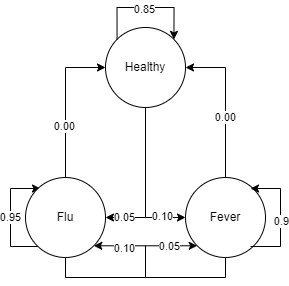
\includegraphics[width=.5\textwidth]{UML0.drawio}
	\end{center}
\end{figure}
\subsection{1 b}
There is some rounding errors in the calculations and numbers, but this will not change the path in this case.
\begin{figure}[!h]
	\begin{center}
		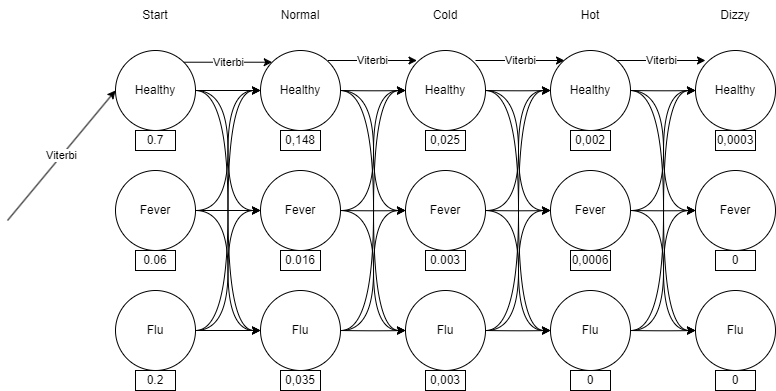
\includegraphics[width=.8\textwidth]{UML1.drawio}
	\end{center}
\end{figure}

\newpage
\section{Generate a set of continuous data given the following table of information}
Generating a set of random given some arguments can be done several ways, after developing three different ways we choose the one which gives the most realistic set.

\begin{itemize}
	\item Random numbers, which can easily comply with the requirements, but is not realistic in any sort of way.
	\item A normal distribution, which do fulfill the requirements and most things, a normal distribution maps to real world, but it doesn't here.
	\item The last one which we used would add points with a certain distance between each other to ensure that we keep most data within the required 75\% data range. The algorithm would then work its way towards the next point with a certain improvement, so it would get closer for each data-point to the targeted point. There would be a chance of going away from the target just to add some noise to the data. [Listing 1]
\end{itemize}

Final data:
\begin{figure}[!h]
	\begin{center}
		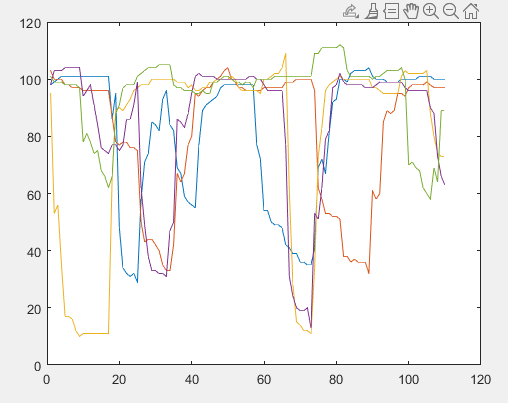
\includegraphics[width=.8\textwidth]{rawData}
	\end{center}
\end{figure}

A data visualizer was also made to run in C\# but was not used due to looking terrible.\\
All requirements are inherently meet except the mean, the mean can be implemented through post-processing by moving some of the datapoints which is outside the 75\% data range either up of down until mean is meet.

\newpage
\section{Develop a machine learning model (HMM) applying the generated dataset}
3.
a. The data is converted into 4 discrete symbols like this:\\
Given value $<$ 36 = 1\\
Given value $>$= 36 and $<$ 65 = 2\\
Given value $>$= 65 and $<$ 94 = 3\\
Given value $>$ 94\\

It is done like this because it is somewhat close to a 4 way split.

b.
\begin{table}[!h]
	\begin{tabular}{|l|l|l|l|}
		\hline
		HMM:         &        &        &        \\ \hline
		pinit\_lrn = &        &        &        \\ \hline
		1.0000       &        &        &        \\ \hline
		0.0000       &        &        &        \\ \hline
		0.0000       &        &        &        \\ \hline
		A\_lrn =     &        &        &        \\ \hline
		0.9573       & 0.0276 & 0.0151 &        \\ \hline
		0.1176       & 0.7954 & 0.0870 &        \\ \hline
		0.0000       & 0.0977 & 0.9023 &        \\ \hline
		B\_lrn1 =    &        &        &        \\ \hline
		0.0000       & 0.0000 & 0.0000 & 1.0000 \\ \hline
		0.0000       & 0.0027 & 0.9672 & 0.0301 \\ \hline
		0.4399       & 0.5577 & 0.0024 & 0.0000 \\ \hline
	\end{tabular}
\end{table}

c.
A bit challeging with the given code, but otherwise not many difficulties.

The more training data and the more discrete symbols used the more accurate the model might become.
However, more training data means more time, and more discrete symbols might make it less general and therefore harder to use.

\begin{table}[!h]
	\noindent\adjustbox{max width=\textwidth}{
		\begin{tabular}{|l|l|l|l|l|l|l|l|l|l|l|l|l|}
		\hline
		Viterbi:                 &        &        &        &        &        &        &        &        &        &        &        &        \\ \hline
		current\_distributions = &        &        &        &        &        &        &        &        &        &        &        &        \\\hline
		0.0000                   &        &        &        &        &        &        &        &        &        &        &        &        \\\hline
		1.0000                   &        &        &        &        &        &        &        &        &        &        &        &        \\\hline
		0.0000                   &        &        &        &        &        &        &        &        &        &        &        &        \\\hline
		all\_distributions =     &        &        &        &        &        &        &        &        &        &        &        &        \\\hline
		Columns 1 through 13     &        &        &        &        &        &        &        &        &        &        &        &        \\\hline
		0.9963                   & 0.9963 & 0.9963 & 0.9963 & 0.9963 & 0.9963 & 0.9963 & 0.9787 & 0.5353 & 0.0000 & 0.0000 & 0.0000 & 0.0000 \\\hline
		0.0037                   & 0.0037 & 0.0037 & 0.0037 & 0.0037 & 0.0037 & 0.0037 & 0.0213 & 0.4647 & 0.9997 & 0.9997 & 0.9997 & 0.9997 \\\hline
		0.0000                   & 0.0000 & 0.0000 & 0.0000 & 0.0000 & 0.0000 & 0.0000 & 0.0000 & 0.0000 & 0.0003 & 0.0003 & 0.0003 & 0.0003 \\\hline
		Columns 14 through 26    &        &        &        &        &        &        &        &        &        &        &        &        \\\hline
		0.0000                   & 0.0000 & 0.0000 & 0.0000 & 0.0000 & 0.0000 & 0.0000 & 0.9963 & 0.9963 & 0.9963 & 0.9963 & 0.9963 & 0.9963 \\\hline
		0.9997                   & 0.9997 & 0.9753 & 0.0378 & 0.9997 & 0.9997 & 1.0000 & 0.0037 & 0.0037 & 0.0037 & 0.0037 & 0.0037 & 0.0037 \\\hline
		0.0003                   & 0.0003 & 0.0247 & 0.9622 & 0.0003 & 0.0003 & 0.0000 & 0.0000 & 0.0000 & 0.0000 & 0.0000 & 0.0000 & 0.0000 \\\hline
		Columns 27 through 39    &        &        &        &        &        &        &        &        &        &        &        &        \\\hline
		0.9963                   & 0.9963 & 0.9963 & 0.9963 & 0.9963 & 0.9963 & 0.9963 & 0.9963 & 0.9963 & 0.9963 & 0.9963 & 0.9963 & 0.9963 \\\hline
		0.0037                   & 0.0037 & 0.0037 & 0.0037 & 0.0037 & 0.0037 & 0.0037 & 0.0037 & 0.0037 & 0.0037 & 0.0037 & 0.0037 & 0.0037 \\\hline
		0.0000                   & 0.0000 & 0.0000 & 0.0000 & 0.0000 & 0.0000 & 0.0000 & 0.0000 & 0.0000 & 0.0000 & 0.0000 & 0.0000 & 0.0000 \\\hline
		Columns 40 through 52    &        &        &        &        &        &        &        &        &        &        &        &        \\\hline
		0.9963                   & 0.9963 & 0.9963 & 0.9963 & 0.9963 & 0.9963 & 0.9963 & 0.9963 & 0.9963 & 0.9963 & 0.9963 & 0.9963 & 0.9963 \\\hline
		0.0037                   & 0.0037 & 0.0037 & 0.0037 & 0.0037 & 0.0037 & 0.0037 & 0.0037 & 0.0037 & 0.0037 & 0.0037 & 0.0037 & 0.0037 \\\hline
		0.0000                   & 0.0000 & 0.0000 & 0.0000 & 0.0000 & 0.0000 & 0.0000 & 0.0000 & 0.0000 & 0.0000 & 0.0000 & 0.0000 & 0.0000 \\\hline
		Columns 53 through 65    &        &        &        &        &        &        &        &        &        &        &        &        \\\hline
		0.9963                   & 0.9963 & 0.9963 & 0.9963 & 0.9963 & 0.9963 & 0.9963 & 0.9963 & 0.9963 & 0.9963 & 0.9963 & 0.9963 & 0.9963 \\\hline
		0.0037                   & 0.0037 & 0.0037 & 0.0037 & 0.0037 & 0.0037 & 0.0037 & 0.0037 & 0.0037 & 0.0037 & 0.0037 & 0.0037 & 0.0037 \\\hline
		0.0000                   & 0.0000 & 0.0000 & 0.0000 & 0.0000 & 0.0000 & 0.0000 & 0.0000 & 0.0000 & 0.0000 & 0.0000 & 0.0000 & 0.0000 \\\hline
		Columns 66 through 78    &        &        &        &        &        &        &        &        &        &        &        &        \\\hline
		0.9963                   & 0.9963 & 0.9963 & 0.9963 & 0.9963 & 0.9963 & 0.9963 & 0.9963 & 0.9963 & 0.9963 & 0.9963 & 0.9963 & 0.9963 \\\hline
		0.0037                   & 0.0037 & 0.0037 & 0.0037 & 0.0037 & 0.0037 & 0.0037 & 0.0037 & 0.0037 & 0.0037 & 0.0037 & 0.0037 & 0.0037 \\\hline
		0.0000                   & 0.0000 & 0.0000 & 0.0000 & 0.0000 & 0.0000 & 0.0000 & 0.0000 & 0.0000 & 0.0000 & 0.0000 & 0.0000 & 0.0000 \\\hline
		Columns 79 through 91    &        &        &        &        &        &        &        &        &        &        &        &        \\\hline
		0.9963                   & 0.9963 & 0.9963 & 0.9963 & 0.9963 & 0.9963 & 0.9963 & 0.9963 & 0.9963 & 0.9963 & 0.9963 & 0.9963 & 0.9963 \\\hline
		0.0037                   & 0.0037 & 0.0037 & 0.0037 & 0.0037 & 0.0037 & 0.0037 & 0.0037 & 0.0037 & 0.0037 & 0.0037 & 0.0037 & 0.0037 \\\hline
		0.0000                   & 0.0000 & 0.0000 & 0.0000 & 0.0000 & 0.0000 & 0.0000 & 0.0000 & 0.0000 & 0.0000 & 0.0000 & 0.0000 & 0.0000 \\\hline
		Columns 92 through 104   &        &        &        &        &        &        &        &        &        &        &        &        \\\hline
		0.9963                   & 0.9963 & 0.9963 & 0.9963 & 0.9963 & 0.9963 & 0.9787 & 0.5353 & 0.0000 & 0.0000 & 0.0000 & 0.0000 & 0.0000 \\\hline
		0.0037                   & 0.0037 & 0.0037 & 0.0037 & 0.0037 & 0.0037 & 0.0213 & 0.4647 & 0.9997 & 0.9997 & 0.9997 & 0.9753 & 0.0005 \\\hline
		0.0000                   & 0.0000 & 0.0000 & 0.0000 & 0.0000 & 0.0000 & 0.0000 & 0.0000 & 0.0003 & 0.0003 & 0.0003 & 0.0247 & 0.9995 \\\hline
		Columns 105 through 110  &        &        &        &        &        &        &        &        &        &        &        &        \\\hline
		0.0000                   & 0.0000 & 0.0000 & 0.0000 & 0.0000 & 0.0000 &        &        &        &        &        &        &        \\\hline
		0.0005                   & 0.0378 & 0.9753 & 0.0378 & 0.9997 & 1.0000 &        &        &        &        &        &        &        \\\hline
		0.9995                   & 0.9622 & 0.0247 & 0.9622 & 0.0003 & 0.0000 &        &        &        &        &        &        &   \\ \hline   
	\end{tabular}
	}

\end{table}

the calculation for the third part of the report are done in the assignment2\_3.m file.

\newpage
\section{Appendix}
Full code: https://github.com/SSpedsbjerg/Reliability

Algorithm used to generate the data sets:
\begin{figure}
	\scriptsize
	\begin{lstlisting}[language=c,caption={Datageneration}]
		class ContinousData : Distrubtion {
			
			double? range0 = null;
			double? range1 = null;
			double requiredDataPercentage = 0;
			
			public void SetTargetRange(double value1, double value2) {
				range0 = value1; range1 = value2;
			}
			
			public void voidTargetRange() {
				range0 = null; range1 = null;
			}
			
			public void setRequiredDataPercentage(double value) {
				requiredDataPercentage = value;
			}
			
			private List<double> GenerateTargetPoints() {
				if(range0 == null || range1 == null) { return null; }
				List<double> points = new List<double>();
				Random random = new Random();
				int totalPoints = (int)((this.GetCount() / 10) + 1);
				for (int i = 0; i < ((requiredDataPercentage / 100) * totalPoints) + 1; i++) {
					points.Add((double)(range0 + (random.NextDouble() * (range1 - range0))));
				}
				for (int i = 0; i <= totalPoints - ((requiredDataPercentage / 100) * totalPoints) + 1; i++) {
					points.Add((double)(this.GetMin() + (random.NextDouble() * (this.GetMax() - this.GetMin()))));
				}
				Shuffel(points);
				return points;
			}
			
			private void Shuffel(List<double> values) {
				Random random = new Random();
				int n = values.Count;
				while(n > 1) {
					n--;
					int k = random.Next(n + 1);
					double value = values[k];
					values[k] = values[n];
					values[n] = value;
				}
			}
			
			public List<double> GenerateData() {
				List<double> points = GenerateTargetPoints();
				List<double> values = new List<double>();
				int i = 0;
				Random random = new Random();
				values.Add(points[i]);
				int j = 0;
				while (this.GetCount() > values.Count()) {
					double maxAddition = ((double)range1 / ((double)range0 + (double)range1));
					try {
						values.Add(values.Last() + ((random.NextDouble() -0.2) * ((points[i + 1] - values.Last()))));
						j++;
						if (j >= (int)((this.GetCount() / points.Count()))) {
							i++;
							Console.WriteLine($"Total Points: {points.Count()}, Points used: {i}");
							j = 0;
							values.Add(points[i]);
						}
					}
					catch(ArgumentOutOfRangeException) {
						Console.WriteLine("Index");
						return values;
					}
				}
				return values;
			}
		}
	\end{lstlisting}
\end{figure}


\end{document}